\documentclass[a4paper,11pt]{article}

% Language setting
\usepackage[french]{babel}

% Page size and margins
\usepackage[top=2cm,bottom=2cm,left=2.2cm,right=2.2cm,marginparwidth=1.75cm]{geometry}

% Useful packages
\usepackage{amsmath}
\usepackage{graphicx}
\usepackage{float}
\usepackage{hyperref}
\hypersetup{colorlinks=true,allcolors=blue}

% Graphics path (images folder is at repo root)
\graphicspath{{../images/}{.}}

% Title
\title{Système de consensus simple pour verrous distribués\\\large Projet ICT3 n°2 — Shanghai Jiao Tong University}
\author{Alexandra Baron \and Maria Stivala \and Mathis Liens \and Arnaud \and Charles \and Baptiste Halçaren}
\date{Octobre 2025}

\begin{document}

% University logo
\begin{figure}[H]
\centering

\includegraphics[width=0.55\linewidth]{shanghai-jiao-tong-university.png}
\end{figure}

\maketitle

\begin{abstract}
Ce rapport présente la conception et l'implémentation d'un système de consensus simple permettant de gérer des verrous distribués avec un serveur chef (leader) et plusieurs serveurs suiveurs (followers). L'implémentation, réalisée en \texttt{Java} sur sockets, garantit la cohérence forte des données: toutes les opérations de \emph{lock}/\emph{unlock} sont validées par le leader puis répliquées à l'ensemble des followers, tandis que les requêtes \emph{own} (lecture) sont servies localement par tout serveur. Nous décrivons l'objectif du projet, la méthode utilisée, l'architecture et la structure du code, puis nous présentons des résultats expérimentaux et discutons des limites.
\end{abstract}

\section{Contexte et objectif}
Dans le cadre du cours ICT3 (Information and Communication Technologies), l'objectif était de \textbf{concevoir un système de consensus simple} répondant aux exigences suivantes: (i) un leader et plusieurs followers; (ii) une \textit{map} répliquée clé\,$\rightarrow$\,propriétaire pour les verrous; (iii) des clients multiples pouvant \texttt{tryLock}, \texttt{tryUnLock} et \texttt{ownTheLock}; (iv) \textbf{toutes} les opérations de mutation (\texttt{LOCK}/\texttt{UNLOCK}) sont routées vers le leader; (v) les lectures (\texttt{OWN}) peuvent être servies localement par les followers; (vi) le leader met à jour sa map et \textbf{propage une proposition} de mise à jour à tous les followers.

\section{Méthode et choix d'implémentation}
Nous avons opté pour une \textbf{architecture leader–followers} au-dessus de sockets TCP Java :\\[-0.6em]
\begin{itemize}
\item \textbf{Protocole texte} minimaliste: \texttt{LOCK,<lockName>,<clientId>}, \texttt{UNLOCK,<lockName>,<clientId>}, \texttt{OWN,<lockName>,<clientId>}.\\
\item \textbf{Routage}: les followers transfèrent \texttt{LOCK}/\texttt{UNLOCK} au leader; \texttt{OWN} est traité localement.\\
\item \textbf{Réplication}: le leader envoie \texttt{SYNC,<cmd>,<lockName>,<clientId>} à tous les followers et attend un \texttt{ACK}.\\
\item \textbf{Tolérance simple aux erreurs}: délais d'attente (5–10s) et codes de retour explicites (\texttt{SUCCESS}/\texttt{FAIL}/\texttt{NONE}/\texttt{ERROR}/\texttt{TIMEOUT}).
\end{itemize}

\section{Architecture fonctionnelle}
Le système se compose de trois rôles: client, leader et followers. Les interactions principales sont :
\begin{enumerate}
\item \textbf{LOCK/UNLOCK}: Client $\rightarrow$ Follower $\rightarrow$ Leader $\rightarrow$ Followers (SYNC) $\rightarrow$ Client.
\item \textbf{OWN}: Client $\rightarrow$ (n'importe quel) Serveur $\rightarrow$ Client.
\end{enumerate}
La cohérence est assurée par l'ordonnancement des mutations au leader et la réplication synchrone via messages \texttt{SYNC}.

\section{Structure du code}
Le dépôt contient trois classes Java principales:
\begin{itemize}
\item \textbf{\texttt{Server.java}}: écoute sur un port TCP, gère les connexions en pool de threads, décide au leader des règles métier (succès/échec de \texttt{LOCK}/\texttt{UNLOCK}), maintient \texttt{lockMap} et notifie les followers avec \texttt{SYNC}. Côté follower, transfère \texttt{LOCK}/\texttt{UNLOCK} au leader et répond localement aux \texttt{OWN}.
\item \textbf{\texttt{Client.java}}: expose \texttt{tryLock}, \texttt{tryUnLock}, \texttt{ownTheLock}, envoie un message puis lit la réponse sur une nouvelle connexion TCP par opération.
\item \textbf{\texttt{DistributedLockTest.java}}: scénarios multi-clients et multi-serveurs (leader 10.0.2.3, followers 10.0.2.4 / 10.0.2.5) pour vérifier acquisition concurrente, lecture du propriétaire et libération.
\end{itemize}

\subsection*{Règles métier}
\begin{itemize}
\item \textbf{Préemption (LOCK)}: succès si le verrou n'existe pas; sinon échec.
\item \textbf{Libération (UNLOCK)}: succès si l'appelant est propriétaire; sinon échec.
\item \textbf{Lecture (OWN)}: tout client peut connaître le propriétaire (ou \texttt{NONE}).
\end{itemize}

\section{Protocole et messages}
\begin{center}
\begin{tabular}{|l|l|l|}
\hline
\textbf{Type} & \textbf{Format} & \textbf{Description}\\\hline
Client $\rightarrow$ Serveur & \texttt{LOCK,\$name,\$client} & Acquisition de verrou\\\hline
Client $\rightarrow$ Serveur & \texttt{UNLOCK,\$name,\$client} & Libération de verrou\\\hline
Client/Serveur & \texttt{OWN,\$name,\$client} & Lecture du propriétaire\\\hline
Leader $\rightarrow$ Followers & \texttt{SYNC,\$cmd,\$name,\$client} & Réplication de l'état\\\hline
Followers $\rightarrow$ Leader & \texttt{ACK} & Accusé de réception\\\hline
\end{tabular}
\end{center}

\section{Résultats expérimentaux}
Les figures suivantes illustrent le démarrage des trois serveurs, l'exécution du test automatisé et la connexion simultanée de deux clients.

\begin{figure}[H]
\centering
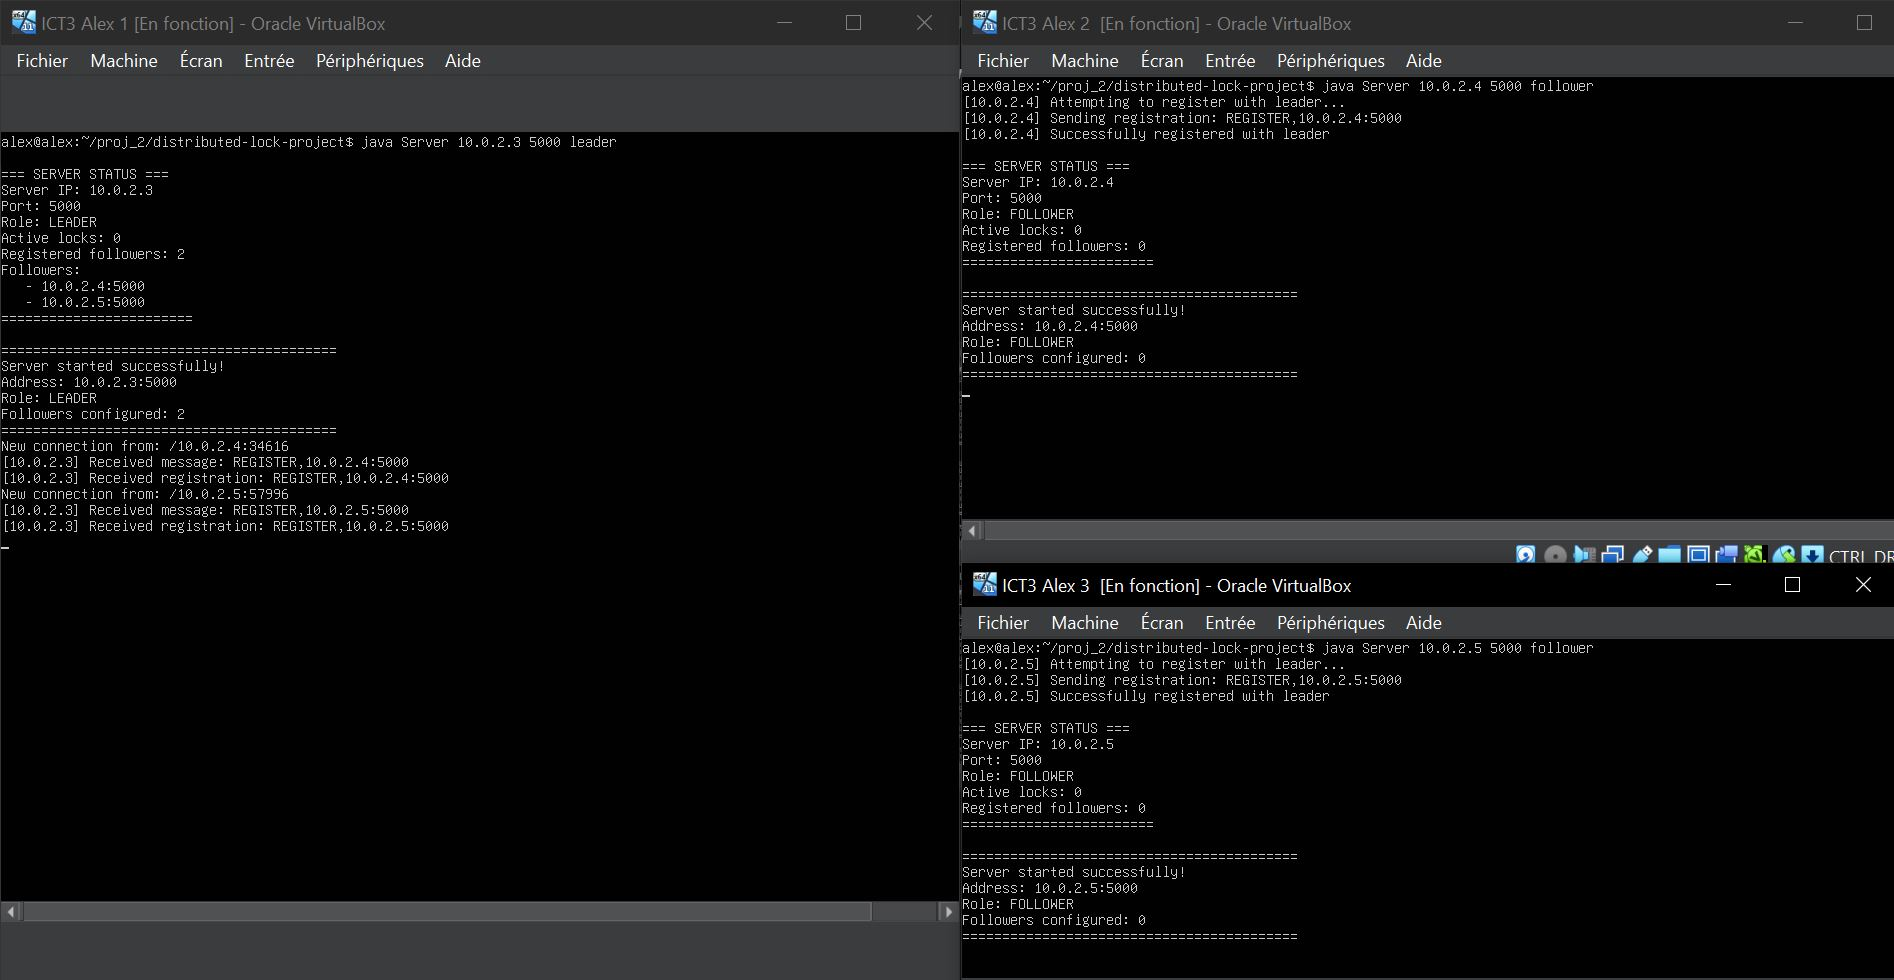
\includegraphics[width=0.9\linewidth]{Capture_connection des 3 serveurs .JPG}
\caption{Initialisation du leader et des deux followers.}
\end{figure}

\begin{figure}[H]
\centering
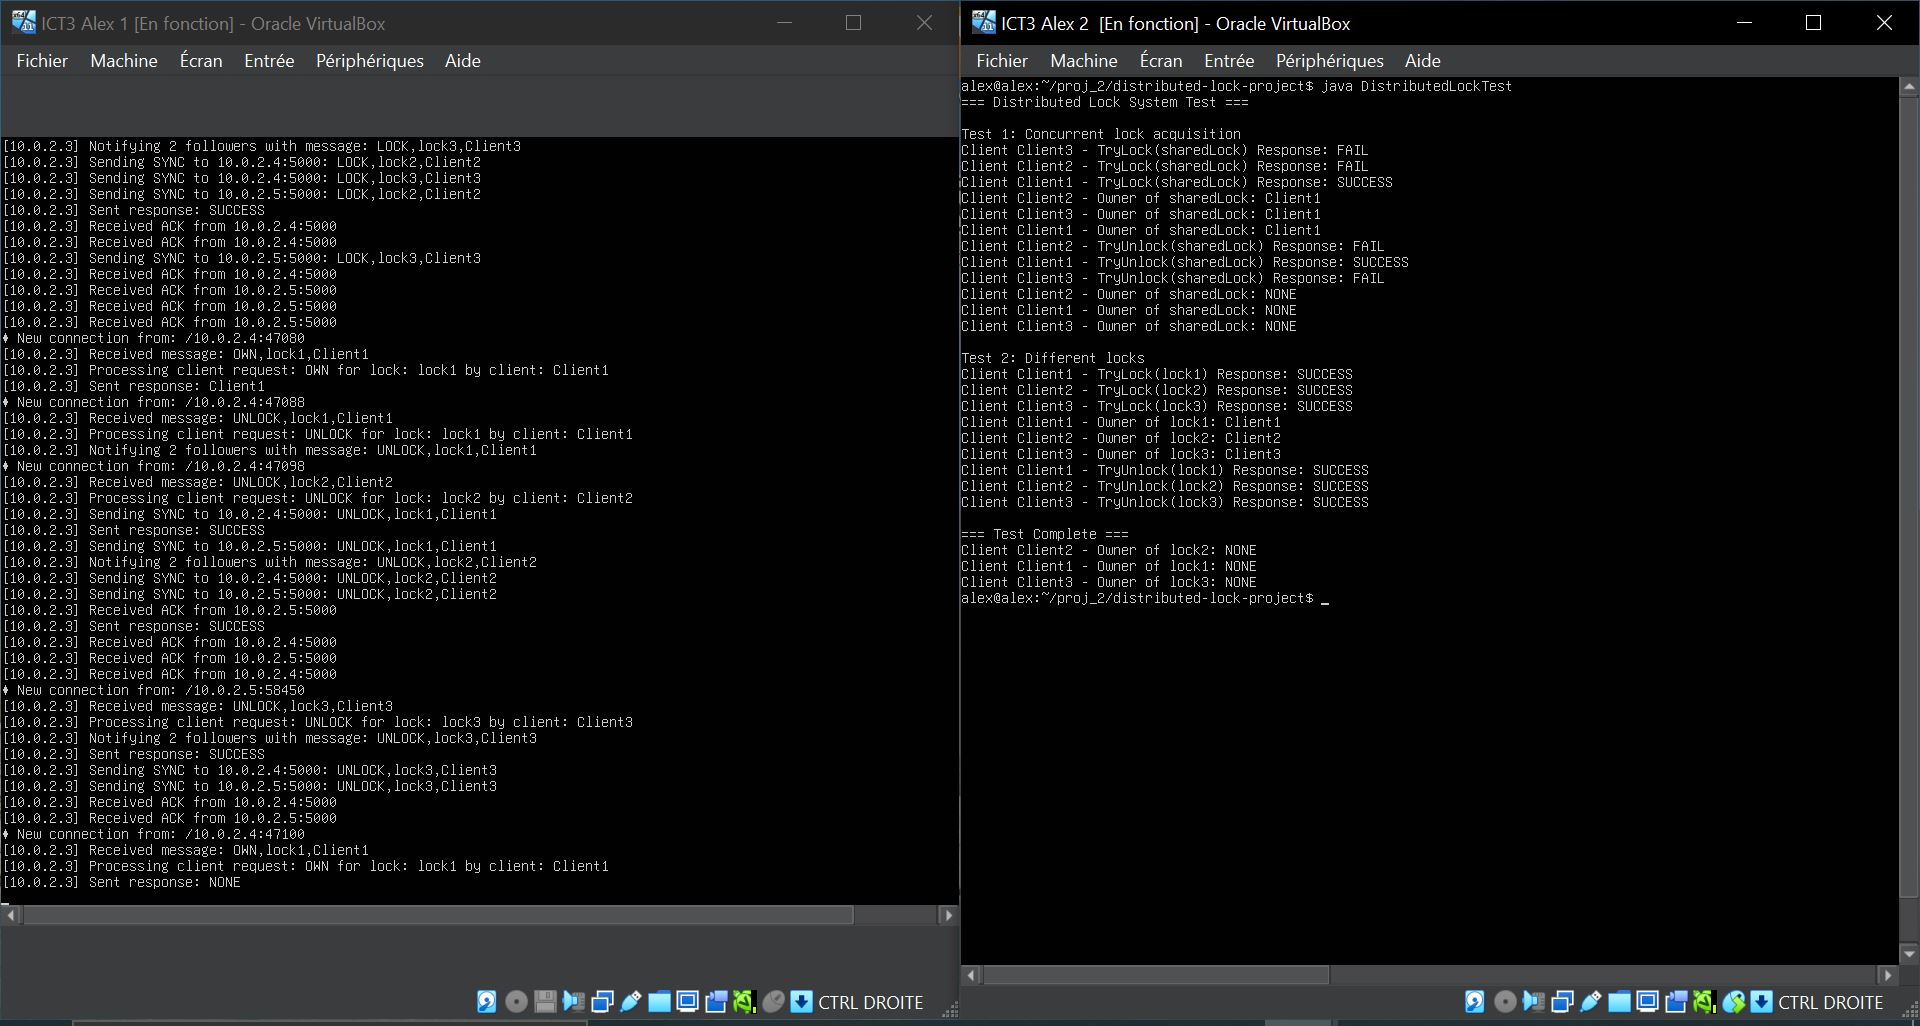
\includegraphics[width=0.9\linewidth]{Capture_distributed_lock_test.JPG}
\caption{Exécution de \texttt{DistributedLockTest}: acquisitions, lectures, libérations.}
\end{figure}

\begin{figure}[H]
\centering
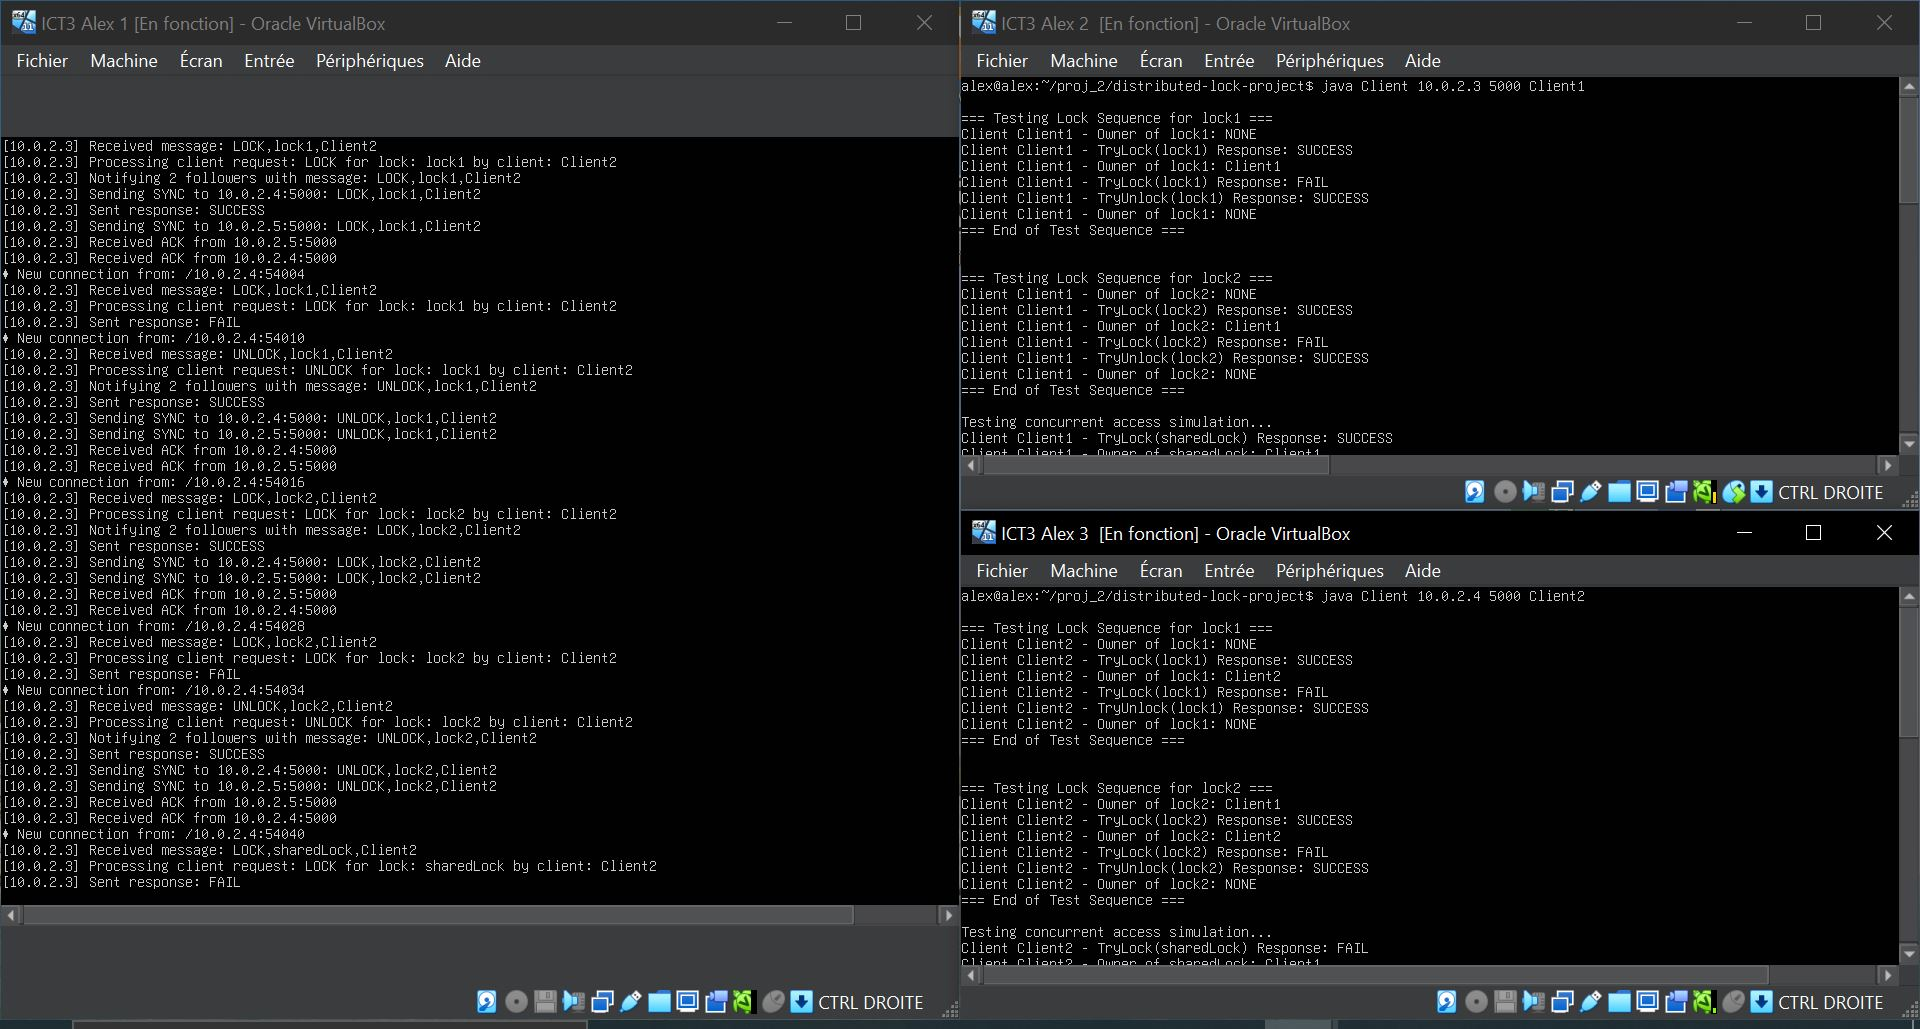
\includegraphics[width=0.9\linewidth]{Capture_ connection de deux clients .JPG}
\caption{Connexion concurrente de deux clients sur des serveurs distincts.}
\end{figure}

\subsection*{Observations}
\begin{itemize}
\item Une seule acquisition réussit sur un même verrou; les autres tentatives échouent (\texttt{FAIL}).
\item Les lectures \texttt{OWN} retournent le propriétaire attendu ou \texttt{NONE} après libération.
\item La réplication \texttt{SYNC} maintient la cohérence entre leader et followers.
\end{itemize}

\section{Limites et pistes d'amélioration}
\begin{itemize}
\item \textbf{Suivi d'état ``pending''}: non implémenté côté followers; l'ajout d'une file de requêtes permettrait d'adhérer mot-à-mot au sujet.
\item \textbf{Paramétrage réseau}: l'adresse du leader est codée en dur (10.0.2.3). Un fichier de configuration ou des arguments CL seraient préférables.
\item \textbf{Robustesse}: pas d'élection de leader ni reprise automatique; hors périmètre du sujet mais envisageable.
\end{itemize}

\section{Conclusion}
Nous avons réalisé un système de verrous distribués conforme aux exigences essentielles du sujet: un leader, plusieurs followers, réplication consistante, et un protocole simple sur sockets avec trois opérations client. Les tests démontrent la cohérence de l'état et la bonne application des règles métier. Ce socle peut servir de base à des extensions (file \emph{pending}, configuration dynamique, sécurité, élection de leader).

\end{document}
